%% This style is provided for the ICSE 2015 main conference,
%% ICSE 2015 co-located events, and ICSE 2015 workshops.

%% bare_conf_ICSE15.tex
%% V1.4
%% 2014/05/22


%% This is a skeleton file demonstrating the use of IEEEtran.cls
%% (requires IEEEtran.cls version 1.7 or later) with an IEEE conference paper.
%%
%% Support sites:
%% http://www.michaelshell.org/tex/ieeetran/
%% http://www.ctan.org/tex-archive/macros/latex/contrib/IEEEtran/
%% and
%% http://www.ieee.org/

%%*************************************************************************
%% Legal Notice:
%% This code is offered as-is without any warranty either expressed or
%% implied; without even the implied warranty of MERCHANTABILITY or
%% FITNESS FOR A PARTICULAR PURPOSE!
%% User assumes all risk.
%% In no event shall IEEE or any contributor to this code be liable for
%% any damages or losses, including, but not limited to, incidental,
%% consequential, or any other damages, resulting from the use or misuse
%% of any information contained here.
%%
%% All comments are the opinions of their respective authors and are not
%% necessarily endorsed by the IEEE.
%%
%% This work is distributed under the LaTeX Project Public License (LPPL)
%% ( http://www.latex-project.org/ ) version 1.3, and may be freely used,
%% distributed and modified. A copy of the LPPL, version 1.3, is included
%% in the base LaTeX documentation of all distributions of LaTeX released
%% 2003/12/01 or later.
%% Retain all contribution notices and credits.
%% ** Modified files should be clearly indicated as such, including  **
%% ** renaming them and changing author support contact information. **
%%
%% File list of work: IEEEtran.cls, IEEEtran_HOWTO.pdf, bare_adv.tex,
%%                    bare_conf.tex, bare_jrnl.tex, bare_jrnl_compsoc.tex
%%*************************************************************************

% *** Authors should verify (and, if needed, correct) their LaTeX system  ***
% *** with the testflow diagnostic prior to trusting their LaTeX platform ***
% *** with production work. IEEE's font choices can trigger bugs that do  ***
% *** not appear when using other class files.                            ***
% The testflow support page is at:
% http://www.michaelshell.org/tex/testflow/



% Note that the a4paper option is mainly intended so that authors in
% countries using A4 can easily print to A4 and see how their papers will
% look in print - the typesetting of the document will not typically be
% affected with changes in paper size (but the bottom and side margins will).
% Use the testflow package mentioned above to verify correct handling of
% both paper sizes by the user's LaTeX system.
%
% Also note that the "draftcls" or "draftclsnofoot", not "draft", option
% should be used if it is desired that the figures are to be displayed in
% draft mode.
%
\documentclass[conference]{IEEEtran}
 
\hyphenation{op-tical net-works semi-conduc-tor}
\usepackage{times}
\usepackage{url}
\usepackage{graphicx}


\begin{document}
%
% paper title
% can use linebreaks \\ within to get better formatting as desired
\title{The Art and Science of Analyzing Software Data; Quantitative Methods}


% author names and affiliations
% use a multiple column layout for up to three different
% affiliations
%\author{\IEEEauthorblockN{Michael Shell}
%\IEEEauthorblockA{School of Electrical and\\Computer Engineering\\
%Georgia Institute of Technology\\
%Atlanta, Georgia 30332--0250\\
%Email: http://www.michaelshell.org/contact.html}
%\and
%\IEEEauthorblockN{Homer Simpson}
%\IEEEauthorblockA{Twentieth Century Fox\\
%Springfield, USA\\
%Email: homer@thesimpsons.com}
%\and
%\IEEEauthorblockN{James Kirk\\ and Montgomery Scott}
%\IEEEauthorblockA{Starfleet Academy\\
%San Francisco, California 96678-2391\\
%Telephone: (800) 555--1212\\
%Fax: (888) 555--1212}}

% conference papers do not typically use \thanks and this command
% is locked out in conference mode. If really needed, such as for
% the acknowledgment of grants, issue a \IEEEoverridecommandlockouts
% after \documentclass

% for over three affiliations, or if they all won't fit within the width
% of the page, use this alternative format:
% 
\author{% 
Tim Menzies\\
Computer Science, \\
North Carolina State University, USA\\
tim.menzies@gmail.com
\and
 Leandro Minku\\
Comptuer Science\\
University of Birmingham, UK\\
l.l.minku@cs.bham.ac.uk
\and
Fayola Peters\\
Lero, University \\of Limmerick, Ireland\\
fayolapeters@gmail.com
}




% use for special paper notices
%\IEEEspecialpapernotice{(Invited Paper)}




% make the title area
 \IEEEspecialpapernotice{(ICSE Technical Briefing)} 
\maketitle


\begin{abstract}
%\boldmath
Using the tools of quantitative data science, software engineers that can predict useful information on new projects based on past projects.  This tutorial reflects on the state-of-the-art in quantitative  reasoning in this important field. This  tutorial discusses the following:   (a) when local data is scarce, we show how to adapt data from other organizations to local problems; (b) when working with data of dubious quality, we show how to prune spurious information; (c) when data or models seem too complex, we show how to simplify   data mining results; (d) when the world changes, and old models need to be updated, we show how to handle those updates; (e) when the effect is too complex for one model, we show to how reason over ensembles.
\end{abstract}
% IEEEtran.cls defaults to using nonbold math in the Abstract.
% This preserves the distinction between vectors and scalars. However,
% if the conference you are submitting to favors bold math in the abstract,
% then you can use LaTeX's standard command \boldmath at the very start
% of the abstract to achieve this. Many IEEE journals/conferences frown on
% math in the abstract anyway.

% no keywords




% For peer review papers, you can put extra information on the cover
% page as needed:
% \ifCLASSOPTIONpeerreview
% \begin{center} \bfseries EDICS Category: 3-BBND \end{center}
% \fi
%
% For peerreview papers, this IEEEtran command inserts a page break and
% creates the second title. It will be ignored for other modes.
\IEEEpeerreviewmaketitle
 
 \section{Overview}
 In the age of big data, data science for software engineering is a very active area.  In the 21st century, it is now impossible to manually browse all the available software project data. The PROMISE repository of SE data has grown to 100+ projects and this is just one of over a dozen open-source repositories that are readily available to researchers. There are many sources of information; e.g. example, as of October 2012, Mozilla Firefox had 800K reports on projects; and Source-forge.net Github host 324K and 11.2M projects.


There are many successful results in this field (see Figure 1).
       These results have inspired much interest in this kind of data analysis in the industrial and research communities. A search through Amazon.com reveals dozens of new data mining texts, just in the last 2 years.  Yet most of those texts are overly concerned with the specific details of particular data miners. Industrial practitioners should be able to use a range of approaches as decision support tools which allow prediction of useful information on new software projects based on completed projects. 
       
This tutorial is our reflection  and summary
on the state-of-the-art in quantitative reasoning in this important field. For further information, see our
recent book on this topic (see Figure~2).

\section{Details}   
       
{\em  Target audience: }Software practitioners and researchers wanting to understand the state of the art in using data mining for software engineering (SE) data.  
 
{\em Pre-requisites:} This tutorial makes minimal use of maths of advanced algorithms and would be understandable by  developers and technical managers. 
 


\begin{figure}[!t]
\begin{tabular}{|p{.95\linewidth}|}\hline
  Christian Bird found that it was  possible to build high-quality software using teams across the planet, just as long as the management is structured around code functionality (who works on what) and not merely on geography (who sits where)~\cite{bird09a}.

Another result from AT\&T~\cite{ostrand04} (which has been repeated several times~\cite{me10a,tosun10}) is that static code measures can be used to guide inspection teams to the small parts of the code containing most defects; e.g. inspection teams can find 80\% to 88\% of the defects after inspecting 20\% to 25\% of the code. 
 
For more examples, see the long list of applications discussed in the July and September 2013 issues of IEEE Software special issues on “Software Analytics”, edited by Menzies \& Zimemrmann.
\\\hline
\end{tabular}
\caption{Successful results, analyzing software data.}
\end{figure}
\begin{figure}[!t]
\centering
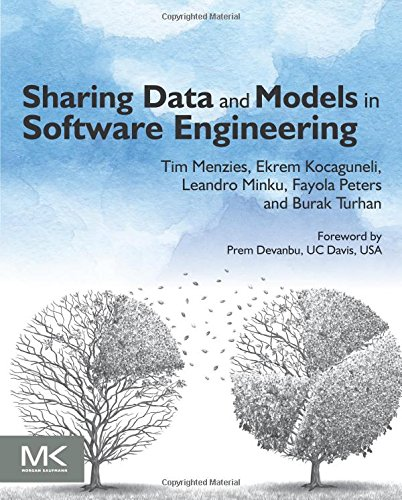
\includegraphics[width=2.65in]{book.jpg}
\caption{Sharing Data and Models,
available from Amazon.com.}
\label{fig:book}
\end{figure}
 
{\em Overall goal of the tutorial:} Better data mining by better skilled software engineers.


{\em Why the topic would be of interest to a broad section of the software engineering community:} 

  We show how to acquire knowledge from software engineering data, so that software engineers can make informed decisions.
\section{About the Presenters}

Tim Menzies (Ph.D., UNSW, 1995) is a full Professor in Computer Science at North Carolina State University where he teaches software engineering and automated software engineering. His research relates to synergies between human and artificial intelligence, with particular application to data mining for software engineering.
He is the author of over 230 referred publications; and is one of the 100 most cited authors in software engineering out of over 80,000 researchers (http://goo.gl/SSPX3J). In his career, he has been a lead researcher on projects for NSF, NIJ, DoD, NASA, USDA, as well as joint research work with private companies.
Prof. Menzies is the co-founder of the PROMISE conference series devoted to reproducible experiments in software engineering (http://openscience.us/repo). He is an associate editor of IEEE Transactions on Software Engineering, Empirical Software Engineering and the Automated Software Engineering Journal. In 2016, he will serve as co-general chair for ICSME'16.


Leandro L. Minku is a Research Fellow II at the Centre of Excellence for Research in Computational Intelligence and Applications (CERCIA), School of Computer Science, the University of Birmingham (UK). He received the PhD degree in Computer Science from the University of Birmingham (UK) in 2011, and was an intern at Google Zurich for six months in 2009/2010. He was the recipient of the Overseas Research Students Award (ORSAS) from the British government and several scholarships from the Brazilian Council for Scientific and Technological Development (CNPq). His research focuses on software prediction models, on-line/incremental machine learning for changing environments, and ensembles of learning machines. He has published in internationally renowned journals such as ACM Transactions on Software Engineering and Methodology, IEEE Transactions on Knowledge and Data Engineering.

Fayola Peters is a Postdoctoral Researcher with Lero - The Irish Software Research Center at the University of Limerick in Ireland. She received the PhD in Computer Science from West Virginia University in 2014. Her research focuses on handling privacy issues related to supporting privacy preserving data sharing for data owners 
(as well as software users). She has published at top software engineering venues like ICSE, IEEE TSE and ESEM. She has also been a curator for the PROMISE repository since 2011.



% trigger a \newpage just before the given reference
% number - used to balance the columns on the last page
% adjust value as needed - may need to be readjusted if
% the document is modified later
%\IEEEtriggeratref{8}
% The "triggered" command can be changed if desired:
%\IEEEtriggercmd{\enlargethispage{-5in}}

% references section
\newpage
% can use a bibliography generated by BibTeX as a .bbl file
% BibTeX documentation can be easily obtained at:
% http://www.ctan.org/tex-archive/biblio/bibtex/contrib/doc/
% The IEEEtran BibTeX style support page is at:
% http://www.michaelshell.org/tex/ieeetran/bibtex/
\bibliographystyle{plain}
% argument is your BibTeX string definitions and bibliography database(s)
\bibliography{refs}
%
% <OR> manually copy in the resultant .bbl file
% set second argument of \begin to the number of references
% (used to reserve space for the reference number labels box)
 




% that's all folks
\end{document}


